\paragraph{Training source and identity units.}
The primary source is the National Library of Medicine (NLM) Computational Photography Project for Pill Identification (C3PI) collection~\citep{yaniv2016nlm}. Its consumer-image list contains 40,882 entries, including 295 exact repeats, leaving 40,587 distinct photographs that were successfully cropped and assigned to partitions. Pill types are defined by nine-digit National Drug Code (NDC9) and product part, giving 2,400 types after package variants are consolidated. Types sharing recorded imprint, shape, colour and size form an \emph{appearance group}, while those without imprint text remain separate. The resulting 2,338 groups define training labels and partition membership, with product identities retained for catalogue retrieval.

Consumer photographs vary in illumination, orientation, visible side and background, with a median of 15 images per medicine and a range of 3--101 in the inventory's NDC9 summary. Studio references provide more consistent views for catalogue matching and augment training groups in runs 3 and 4. Appendix~\ref{app:data} details the count reconciliation, package variants and grouping process, together with the distribution plot in Figure~\ref{fig:data-statistics}.

\begin{table}[!htbp]
\centering\small
\caption{C3PI partitions after removal of repeated entries and successful cropping of all 40,587 distinct consumer photographs. Studio references add 6,198 training crops in runs 3 and 4.}
\label{tab:data}
\begin{tabular}{@{}lrrl@{}}
\toprule
Partition & Groups & Crops & Role \\
\midrule
Training & 1,710 & 29,471 & Representation learning \\
Validation enrolled & 214 & 3,556 & Selection and enrolment \\
Validation unknown & 214 & 3,555 & Rejection calibration \\
Held-out test & 200 & 4,005 & Evaluation on unseen groups \\
\bottomrule
\end{tabular}
\end{table}

\paragraph{Partitioning and preprocessing.}
Groups containing an ePillID fold-4 holdout identity are reserved through NDC9 matching. Remaining groups are randomly divided approximately 80:10:10 between training and the two validation partitions (Table~\ref{tab:data}). Code for split generation checks shared identifiers, exact duplicates and near-duplicate crops. Only references for training groups are added in runs 3 and 4. Each detected pill is framed in a square window of 1.55 times the long side of its bounding box and resized to $224\times224$ pixels. VGG16 inputs use ImageNet channel statistics, while ViT inputs are scaled to $[-1,1]$, with constants given in Appendix~\ref{app:configuration}. Training augmentation is specified in Section~\ref{sec:training}. Figure~\ref{fig:examples} provides representative views.



\begin{figure}[!htbp]
\centering
\begin{minipage}[t]{0.48\linewidth}
\vspace{0pt}\centering
\textbf{(a) C3PI image variation}\\[3pt]
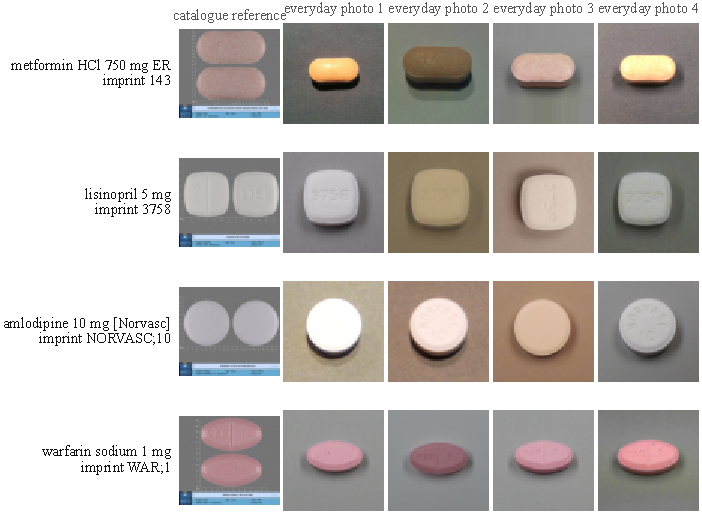
\includegraphics[width=\linewidth]{fig04_qualitative_examples.pdf}
\end{minipage}\hfill
\begin{minipage}[t]{0.49\linewidth}
\vspace{0pt}\centering
\textbf{(b) ePillID side coverage}\\[3pt]
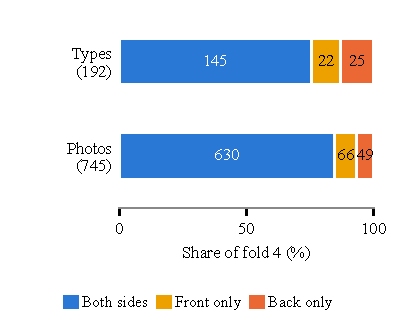
\includegraphics[width=\linewidth]{figD4_epillid_sides_compact.pdf}
\end{minipage}
\caption{Data characteristics. (a) Catalogue references and four consumer photographs for each of four medicines illustrate variation in orientation, visible side and illumination. (b) ePillID fold-4 coverage by side availability, shown for pill types and photographs.}
\label{fig:examples}
\end{figure}

\paragraph{Evaluation sources and catalogue.}
The C3PI holdout comprises 200 appearance groups, whereas the local ePillID release contains 13,532 images of 4,902 types, including 9,804 references and 3,728 consumer images. Fold 4 contains 745 consumer photographs of 192 identities~\citep{usuyama2020epillid}. The official ePillID protocol permits reference images for test types during training, distinguishing it from the strict C3PI evaluation. MEDISEG~\citep{mediseg2026} contributes 8,261 images with 14,069 annotated pills from 32 Hong Kong products. For evaluation with all products enrolled, three single-pill photographs per product form the gallery, leaving 13,973 query pills after 96 enrolment instances are excluded. The median pill long side is 81 pixels, with fifth and 95th percentiles of 27 and 194 pixels in $640\times640$ images. A separate deployment subset has 40 query pills. Product population, scale, cameras and clutter change together, so the external gap cannot be attributed to camera hardware alone. Catalogue identification uses 4,936 US products assembled from C3PI reference images and imprint, shape and colour metadata.

\paragraph{Data use.}
The study uses public image datasets without patient records. C3PI images are restricted to research and development, including when accessed through ePillID, whose MIT code licence does not supersede the image conditions. MEDISEG is distributed under CC BY 4.0, and download instructions for all sources are provided in \texttt{epills/docs/datasets.md}.
